% !TeX spellcheck = en_US
\documentclass[12pt]{article}

% Language setting
\usepackage[english]{babel}

% Set page size and margins
\usepackage[
  a4paper,
  top=2cm,
  bottom=3cm,
  left=2cm,
  right=2cm,
  marginparwidth=1.75cm,
  footskip=2.05cm
]{geometry}

% Useful packages
\usepackage[export]{adjustbox}
\usepackage{amsmath}
\usepackage{caption}
\usepackage[strict]{changepage}
\usepackage{enumitem}
\usepackage{float}
\usepackage{fullwidth}
\usepackage{graphicx, trimclip}
\usepackage[colorlinks=true, allcolors=blue]{hyperref}
\usepackage{hyperref}
\usepackage[nonewpage]{imakeidx}
\usepackage{multicol}
\usepackage{outlines}
\usepackage{setspace}
\usepackage{stfloats}
\usepackage{subfigure}
\usepackage[usetransparent=false]{svg}
\usepackage[subfigure]{tocloft}
\usepackage{tikz}
\usepackage{titlesec}
\usepackage{varwidth}
\usepackage{wrapfig}
\usepackage[most]{tcolorbox}
\newtcolorbox{scaledfigure}[1][]{height fill, space to=\myspace,#1}
\hypersetup{
  colorlinks=true,
  linkcolor=goldenbrown,
  filecolor=magenta,
  urlcolor=cyan,
  pdftitle={Heroes of Might \& Magic III Components List},
  pdfpagemode=UseNone,
}
% Set the default spacing between paragraphs. Remove indentation.
\usepackage[skip=6pt, indent=0pt]{parskip}
\setstretch{1}

% Add dots to the table of contents
\renewcommand{\cftsecleader}{\cftdotfill{\cftsecdotsep}}
\renewcommand\cftsecdotsep{\cftdot}
\renewcommand\cftsubsecdotsep{\cftdot}

\captionsetup[figure]{labelformat=empty}
\usetikzlibrary{shadows, shadows.blur, calc}

\setlength{\columnsep}{1cm}

% Variables
\def\_assets{assets}

\def\art{\_assets/art}
\def\cards{\_assets/cards}
\def\examples{\_assets/examples}
\def\images{\_assets/images}
\def\layout{\_assets/layout}
\def\map_locations{\_assets/map-locations}
\def\skills{\_assets/skills}
\def\spells{\_assets/spells}
\def\svgs{\_assets/glyphs}
\def\notes_svgs{\svgs/for-notes}
\def\tables{\_assets/tables}
\def\qr{\_assets/qr-codes}
\def\covers{\_assets/box-covers}

% Colors
\definecolor{darkcandyapplered}{rgb}{0.64, 0.0, 0.0}
\definecolor{antiquewhite}{rgb}{0.98, 0.92, 0.84}
\definecolor{goldenbrown}{rgb}{0.6, 0.4, 0.08}
\definecolor{arylideyellow}{rgb}{0.91, 0.84, 0.42}
\definecolor{amber}{rgb}{1.0, 0.49, 0.0}

% Command to frame images
\newcommand\framedimage[2][]{%
  \begin{tikzpicture}
    \draw (0, 0) node[inner sep=0] {\makebox[#1][c]{\includegraphics[width=#1]{#2}}};
    \draw [borderoutyellow, thick] (current bounding box.north west) rectangle (current bounding box.south east);
  \end{tikzpicture}}
% End of drop frame definition

\titleformat{\section}
{\huge}
{\filright
\footnotesize
\enspace SECTION \thesection\enspace}
{8pt}
{\Huge\bfseries\filcenter\uppercase}
%Create section heading with graphics. Argument one is heading name, argument two is picture to use on the left.
\newcommand{\addsection}[2]{
  \vspace*{-5em}
  \hspace*{-1em}
  \makebox[0pt][l]{
  \raisebox{-\totalheight}[0pt][7pt]{
    \begin{tikzpicture}
      \draw (0, 0) node[inner sep=0] {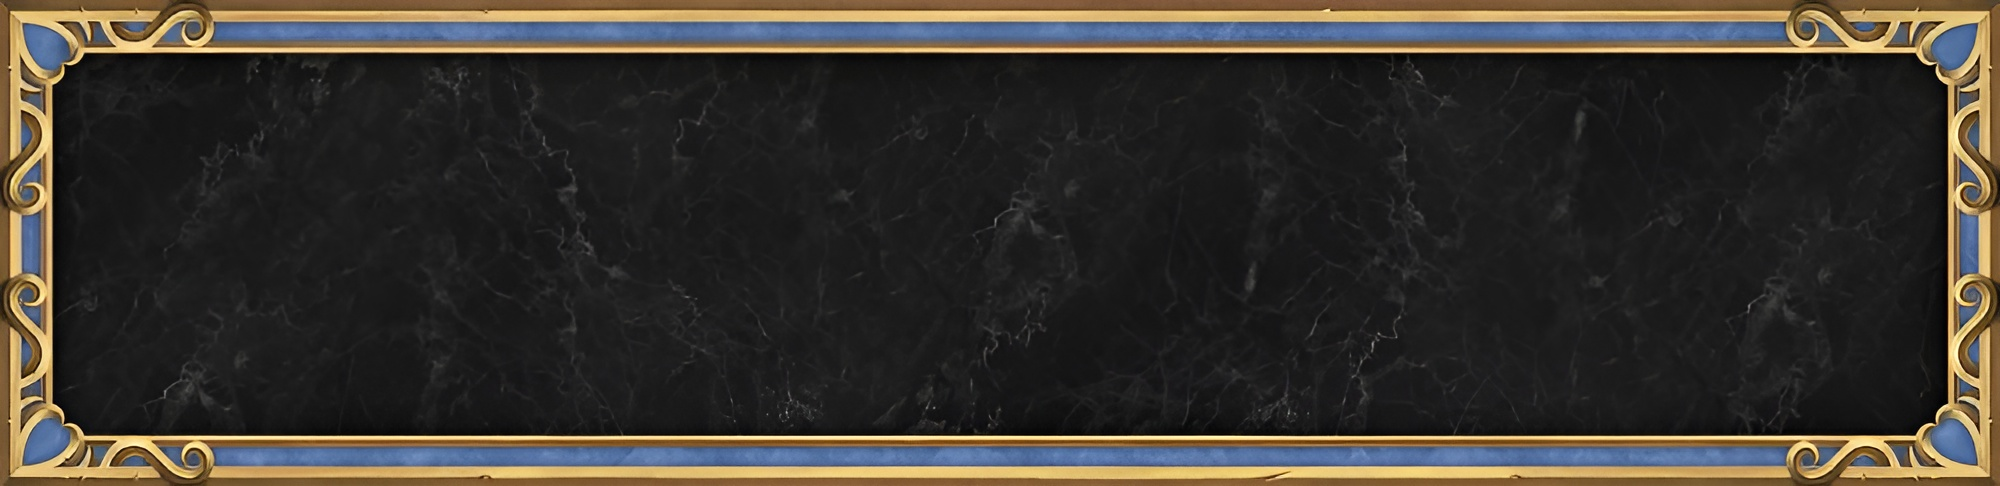
\includegraphics[width=\linewidth, height=0.2\linewidth]{\layout/section_heading.jpg}};
      \draw (-6.2, 0) node {\framedimage[0.14\textwidth]{#2}};
    \end{tikzpicture}
    }
  }
  \begin{fullwidth}[leftmargin=0.16\textwidth]
    \begin{center}
      \fontfamily{ptm}\selectfont{
        \color{antiquewhite} \section*{#1}
        \cleardoublepage\phantomsection\addcontentsline{toc}{section}{\protect\numberline{}#1}
      }
    \end{center}
  \end{fullwidth}
  \vspace{1.75em}
}
%End of create section heading.

\newcommand\picdims[4][]{%
  \setbox0=\hbox{\includegraphics[#1]{#4}}%
  \clipbox{.5\dimexpr\wd0-#2\relax{} %
    .5\dimexpr\ht0-#3\relax{} %
    .5\dimexpr\wd0-#2\relax{} %
    .5\dimexpr\ht0-#3\relax}{\includegraphics[#1]{#4}}}

\tikzset{
  thick/.style=      {line width=1.3pt},
  very thick/.style= {line width=1.7pt},
  ultra thick/.style={line width=2.2pt}
}

\definecolor{borderoutyellow}{HTML}{E0B75F}
\definecolor{borderinyellow}{HTML}{F6EA48}
% Create note box
\newcommand{\note}[2]{
  \begin{tikzpicture}
    \draw (0, 0) node[inner sep=0] {\makebox[\linewidth][c]{\picdims[width=\linewidth]{\linewidth}{#1\baselineskip}{\layout/note-big.jpg}}};
    \draw [black, ultra thick] ([xshift=+2pt, yshift=-2pt] current bounding box.north west) rectangle ([xshift=-2pt, yshift=2pt] current bounding box.south east);
    \draw [borderoutyellow, very thick] (current bounding box.north west) rectangle (current bounding box.south east);
    \draw [borderinyellow, thick] ([xshift=+4.5pt, yshift=-4.5pt] current bounding box.north west) rectangle ([xshift=-4.5pt, yshift=4.5pt] current bounding box.south east);
    \node at (current bounding box.center) {
      \begin{varwidth}{0.85\linewidth}
      \fontfamily{ptm}\selectfont{
        \color{arylideyellow}
        \hypersetup{linkcolor=amber}
        #2
        \hypersetup{linkcolor=goldenbrown}
      }
      \end{varwidth}
    };
  \end{tikzpicture}
}

% Command for overlay circled text
\definecolor{goblin}{HTML}{3b7c33}
\newcommand\encircle[1]{%
  \tikz[baseline=(X.base)]
  \node (X) [draw=white, shape=circle, inner sep=0, fill=goblin, text=white, blur shadow={shadow blur steps=5}] {\strut \textbf{#1}};%
}

% Background
\AddToHook{shipout/background}{%
  \put (0in,-\paperheight){
\includegraphics[width=\paperwidth,height=\paperheight]{\layout/tausta.png}}%
  \put (0in,-\paperheight){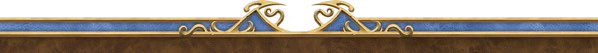
\includegraphics[width=\paperwidth,height=0.05\paperheight]{\layout/bottom.png}}%
}

\makeindex[columns=3, title=, options={-s index_style.ist}]

\title{
\includegraphics[width=6cm]{\images/title.png}\\Components List}

\begin{document}

\maketitle

\begin{center}
  Version 1.0

  \bigbreak
  This document aims to comprehensively list the contents of all the board game boxes.
  It was compiled using a list in \href{https://boardgamegeek.com/thread/3265461/article/43995671#43995671}{this BoardGameGeek thread}.
  \par
  It is a community-driven project, which has a \href{https://github.com/Heegu-sama/Homm3BG}{GitHub repository}.
  Everyone is welcome to contribute, make changes, and fix errors.
\end{center}

\bigbreak

\tableofcontents

\addsection{Core Game}{\covers/core_game.jpg}


\begin{multicols*}{3}

\footnotesize

\begin{itemize}[leftmargin=0pt, label={}, noitemsep]
  \item \textbf{\small{\underline{Books Leaflets}}} (6)
  \item
  \item Player's Aid (3)
  \item Mission Book (1)
  \item Tournament Book (1)
  \item Rule Book (1)
\end{itemize}

\begin{itemize}[leftmargin=0pt, label={}, noitemsep]
  \item \textbf{\small{\underline{Hero Cards}}} (3)
  \item
  \item Catherine/Rion (1)
  \item Mutare/Alamar (1)
  \item Tamika/Sandro (1)
  \item Catherine/Rion (1)
\end{itemize}

\textbf{\small{\underline{Combat Board}}} (1)

\begin{itemize}[leftmargin=0pt, label={}, noitemsep]
  \item \textbf{\small{\underline{Town Boards}}} (3)
  \item
  \item Castle (1)
  \item Dungeon (1)
  \item Necropolis (1)
\end{itemize}

\textbf{\small{\underline{Round Tracker}}} (1)

\textbf{\small{\underline{Map Tiles}}} (20)\\

C1, C2, F1, F2, F3, F4, F5, F6, F7, F8, F9, N1, N2, N3, N4, N5, N6, S1, S2, S3

\begin{itemize}[leftmargin=0pt, label={}, noitemsep]
  \item \textbf{\small{\underline{Miscellaneous Tokens}}} (120)
  \item
  \item 1 Gold (10)
  \item 3 Gold (13)
  \item 10 Gold (10)
  \item 1 Building material (9)
  \item 3 Building material (12)
  \item 1 Valuable (10)
  \item 3 Valuable (6)
  \item Build tokens (3)
  \item Population tokens (3)
  \item 1/2 Damage (10)
  \item 3/5 Damage (5)
  \item Paralysis/Defense (6)
  \item Spell Book (3)
  \item Movement tokens (17)
  \item Morale (2)
  \item Grail (1)
\end{itemize}
\columnbreak
\begin{itemize}[leftmargin=0pt, label={}, noitemsep]
  \item \textbf{\small{\underline{Acrylic Cubes}}} (100)
  \item
  \item Blue (20)
  \item Purple (20)
  \item Grey (20)
  \item Black (40)
\end{itemize}

\begin{itemize}[leftmargin=0pt, label={}, noitemsep]
  \item \textbf{\small{\underline{Dice}}} (8)
  \item
  \item Attack dice (2)
  \item Resource dice (3)
  \item Treasure dice (3)
\end{itemize}

\begin{itemize}[leftmargin=0pt, label={}, noitemsep]
  \item \textbf{\small{\underline{Miniatures}}} (6)
  \item
  \item Castle Heroes (2 poses)
  \item Dungeon Heroes (2 poses)
  \item Necropolis Heroes (2 poses)
\end{itemize}

\begin{itemize}[leftmargin=0pt, label={}, noitemsep]
  \item \textbf{\small{\underline{Cards}}} (258)
  \item
  \item \textbf{Unit Cards} (21)
  \item
  \item \textbf{Castle} (7)
  \item Halberdiers (1)
  \item Marksmen (1)
  \item Griffins (1)
  \item Crusaders (1)
  \item Zealots (1)
  \item Champions (1)
  \item Archangels (1)
  \item
  \item \textbf{Necropolis} (7)
  \item Skeletons (1)
  \item Zombies (1)
  \item Wraiths (1)
  \item Vampires (1)
  \item Liches (1)
  \item Dread Knights (1)
  \item Ghost Dragons (1)
  \item
  \item \textbf{Dungeon} (7)
  \item Troglodytes (1)
  \item Harpies (1)
  \item Evil Eyes (1)
  \item Medusas (1)
  \item Minotaurs (1)
  \item Manticores (1)
  \item Black Dragons (1)
\columnbreak
  \item \textbf{Neutral Unit Cards} (41)
  \item
  \item \textbf{Bronze} (14)
  \item Boars (1)
  \item Evil Eyes (1)
  \item Griffins (1)
  \item Halberdiers (1)
  \item Halflings (2)
  \item Harpies (1)
  \item Marksmen (1)
  \item Peasants (1)
  \item Rogues (1)
  \item Skeletons (1)
  \item Troglodytes (1)
  \item Wraiths (1)
  \item Zombies (1)
  \item
  \item \textbf{Silver} (11)
  \item Crusaders (1)
  \item Liches (1)
  \item Medusas (1)
  \item Minotaurs (1)
  \item Mummies (2)
  \item Nomads (2)
  \item Sharpshooters (1)
  \item Vampires (1)
  \item Zealots (1)
  \item
  \item \textbf{Gold} (12)
  \item Archangels (1)
  \item Black Dragons (1)
  \item Champions (1)
  \item Diamond Golems (2)
  \item Dread Knights (1)
  \item Enchanters (1)
  \item Ghost Dragons (1)
  \item Gold Golems (2)
  \item Manticores (1)
  \item Trolls (1)
  \item
  \item \textbf{Azure} (4)
  \item Azure Dragons (2)
  \item Crystal Dragons (2)
  \item
  \item \textbf{Wall/Gate Cards} (5)
  \item Arrow Tower (1)
  \item Gate Cards (1)
  \item Wall Cards (3)
\columnbreak
  \item \textbf{Statistics Cards} (24)
  \item Attack (5)
  \item Defense (6)
  \item Knowledge (6)
  \item Power (7)
  \item
  \item \textbf{AI Cards} (20)
  \item Attack V1 (2)
  \item Attack V2 (2)
  \item Cast a spell V1 (4)
  \item Cast a spell V2 (4)
  \item Defense V1 (2)
  \item Defense V2 (2)
  \item Use a skill V1 (2)
  \item Use a skill V2 (2)
  \item
  \item \textbf{Astrologers Proclaim} (19)
  \item Annoying Lizard (1)
  \item Battalion's Stallion (1)
  \item Crazy Wizard (1)
  \item Dead Silence (1)
  \item Fancy Pixie (1)
  \item Fluffy Rabbit (1)
  \item Friendly Beaver (1)
  \item Gold Dragon (1)
  \item Greedy Dragon (1)
  \item Grim Warlock (1)
  \item Groovy Satyr (1)
  \item Isra's Friends (1)
  \item Magic Tortoise (1)
  \item Merry Leprachaun (1)
  \item Profuse Growth (1)
  \item Swift Weasel (1)
  \item Terrible Plague (1)
  \item White Raven (1)
  \item Wild Debauchery (1)
  \item
  \item \textbf{Spells} (46)
  \item Anti-magic (2)
  \item Bless (2)
  \item Blind (2)
  \item Bloodlust (2)
  \item Chain Lightning (2)
  \item Counterstrike (2)
  \item Cure (2)
  \item Curse (2)
  \item Disrupting ray (2)
  \item Fire shield (2)
  \item Fireball (2)
  \item Haste (2)
  \item Lightning bolt (2)
  \item Magic Arrow (6)
  \item Prayer (2)
  \item Resurrection (2)
  \item Slow (2)
  \item Stone skin (2)
  \item Teleport (2)
  \item Town Portal (2)
  \item Weakness (2)
  \item
  \item \textbf{Hero Specialties} (18)
  \item
  \item \textbf{Alamar} (3)
  \item Resurrection I (1)
  \item Resurrection IV (1)
  \item Resurrection VI (1)
  \item
  \item \textbf{Mutare} (3)
  \item Dragons I (1)
  \item Dragons IV (1)
  \item Dragons VI (1)
  \item
  \item \textbf{Sandro} (3)
  \item Cloak of the undead king I (1)
  \item Cloak of the undead king IV (1)
  \item Cloak of the undead king VI (1)
  \item
  \item \textbf{Tamika} (3)
  \item Dread knights I (1)
  \item Dread knights IV (1)
  \item Dread knights VI (1)
  \item
  \item \textbf{Rion} (3)
  \item Battlefield medic I (1)
  \item Battlefield medic IV (1)
  \item Battlefield medic VI (1)
  \item
  \item \textbf{Catherine} (3)
  \item Crusaders I (1)
  \item Crusaders IV (1)
  \item Crusaders VI (1)
  \item
  \item \textbf{Artifacts} (32)
  \item Angel Wings (1)
  \item Armor of Wonder (1)
  \item Blackshard of the Dead Knight (1)
  \item Breastplate of Petrified Wood (1)
  \item Centaur's Axe (1)
  \item Charm of Mana (1)
  \item Dragon Scale Armor (1)
  \item Dragon Scale Shield (1)
  \item Dragon Wing Tabard (1)
  \item Endless Bag of Gold (1)
  \item Endless Sack of Gold (1)
  \item Everflowing Crystal Cloak (1)
  \item Everpouring Vial of Mercury (1)
  \item Head of Legion (1)
  \item Hourglass of the Evil Hour (1)
  \item Inexhaustible Cart of Lumber (1)
  \item Legs of Legion (1)
  \item Loins of Legion (1)
  \item Ogre's Club of Havoc (1)
  \item Red Dragon Flame Tongue (1)
  \item Rib Cage (1)
  \item Sentinel's Shield (1)
  \item Shackles of War (1)
  \item Shield of the Dwarven Lords (1)
  \item Shield of the Yawning Dead (1)
  \item Speculum (1)
  \item Sword of Judgement (1)
  \item Targ of the Rampaging Ogre (1)
  \item Titan's Cuirass (1)
  \item Titan's Gladius (1)
  \item Tunic of the Cyclops King (1)
  \item Vial of Lifeblood (1)
  \item
  \item \textbf{Abilities} (30)
  \item Archery (2)
  \item Armorer (2)
  \item Diplomacy (2)
  \item Estates (2)
  \item Intelligence (2)
  \item Leadership (2)
  \item Logistics (2)
  \item Luck (2)
  \item Mysticism (2)
  \item Necromancy (2)
  \item Offense (2)
  \item Resistance (2)
  \item Sorcery (2)
  \item Tactics (2)
  \item Wisdom (2)
  \item
  \item \textbf{Other} (2)
  \item Core Game Deck Cards (2)
\end{itemize}

\end{multicols*}


\addsection{Rampart}{\covers/rampart.jpg}


\begin{multicols*}{3}

\footnotesize

\begin{itemize}[leftmargin=0pt, label={}, noitemsep, noitemsep]
  \item \textbf{\normalsize{\underline{Books Leaflets}}} (2)
  \item
  \item Player's Aid (1)
  \item Mission Book (1)
\end{itemize}

\begin{itemize}[leftmargin=0pt, label={}, noitemsep, noitemsep]
  \item \textbf{\normalsize{\underline{Hero Cards}}} (1)
  \item
  \item Gelu/Gem (1)
\end{itemize}

\begin{itemize}[leftmargin=0pt, label={}, noitemsep, noitemsep]
  \item \textbf{\normalsize{\underline{Town Boards}}} (1)
  \item
  \item Rampart (1)
\end{itemize}

\textbf{\normalsize{\underline{Map Tiles}}} (7)\\

C3, F10, F11, F12, N7, N8, S4

\begin{itemize}[leftmargin=0pt, label={}, noitemsep, noitemsep]
  \item \textbf{\normalsize{\underline{Miscellaneous Tokens}}} (23)
  \item
  \item 1 Gold (3)
  \item 3 Gold (3)
  \item 10 Gold (3)
  \item 1 Building material (3)
  \item 3 Building material (3)
  \item 1 Valuable (3)
  \item 3 Valuable (1)
  \item Build tokens (1)
  \item Population tokens (1)
  \item Spell Book (1)
  \item Morale (1)
\end{itemize}

\begin{itemize}[leftmargin=0pt, label={}, noitemsep, noitemsep]
  \item \textbf{\normalsize{\underline{Acrylic Cubes}}} (30)
  \item
  \item Green (20)
  \item Black (10)
\end{itemize}

\begin{itemize}[leftmargin=0pt, label={}, noitemsep, noitemsep]
  \item \textbf{\normalsize{\underline{Miniatures}}} (9)
  \item
  \item Rampart Heroes (2 poses)
  \item Centaurs (1)
  \item Dwarves (1)
  \item Elves (1)
  \item Pegasi (1)
  \item Dendroids (1)
  \item Unicorns (1)
  \item Gold dragons (1)
\end{itemize}

\columnbreak

\begin{itemize}[leftmargin=0pt, label={}, noitemsep, noitemsep]
  \item \textbf{\normalsize{\underline{Cards}}} (70)
  \item
  \item \textbf{Unit Cards} (7)
  \item Tower (7)
  \item Centaurs (1)
  \item Dwarves (1)
  \item Elves (1)
  \item Pegasi (1)
  \item Dendroids (1)
  \item Unicorns (1)
  \item Gold dragons (1)
  \item
  \item \textbf{Neutral Unit Cards} (2)
  \item
  \item \textbf{Azure} (2)
  \item Faerie Dragons (2)
  \item
  \item \textbf{Statistics Cards} (7)
  \item Attack (1)
  \item Defense (3)
  \item Knowledge (2)
  \item Power (1)
  \item
  \item \textbf{Astrologers Proclaim} (3)
  \item Ammo Cart (1)
  \item Charlie and His Circus (1)
  \item McGiver (1)
  \item
  \item \textbf{Spells} (20)
  \item Dimension Door (2)
  \item Earthquake (2)
  \item Firewall (2)
  \item Forgetfulness (2)
  \item Magic Arrow (4)
  \item Mirth (2)
  \item Precision (2)
  \item Slayer (2)
  \item Sorrow (2)
  \item
  \item \textbf{Hero Specialties} (6)
  \item
  \item \textbf{Gelu} (3)
  \item Sharpshooters I (1)
  \item Sharpshooters IV (1)
  \item Sharpshooters VI (1)
  \item
  \item \textbf{Gem} (3)
  \item First Aid I (1)
  \item First Aid IV (1)
  \item First Aid VI (1)
  \item
  \item \textbf{Artifacts} (8)
  \item Ambassador's Sash (1)
  \item Buckler of The Gnoll King (1)
  \item Cape of Velocity (1)
  \item Golden Bow (1)
  \item Greater Gnoll's Flail (1)
  \item Inexhaustible Cart of Ore (1)
  \item Ord of Vulnerability (1)
  \item Torso of Legion (1)
  \item
  \item \textbf{Abilities} (4)
  \item Artillery (2)
  \item First Aid (2)
  \item
  \item \textbf{War Machines} (12)
  \item Ammo Cart (4)
  \item Ballista (4)
  \item First Aid Tent (4)
  \item
  \item \textbf{Other} (1)
  \item Rampart Deck Cards (1)
\end{itemize}

\end{multicols*}


\addsection{Fortress}{\covers/fortress.jpg}

\begin{multicols*}{3}

\footnotesize

\begin{itemize}[leftmargin=0pt, label={}, noitemsep]
  \item \textbf{\small{\underline{Books Leaflets}}} (2)
  \item
  \item Player's Aid (1)
  \item Fortress Mission Book (1)
\end{itemize}

\begin{itemize}[leftmargin=0pt, label={}, noitemsep]
  \item \textbf{\small{\underline{Hero Cards}}} (1)
  \item
  \item Wystan/Adrienne (1)
\end{itemize}

\begin{itemize}[leftmargin=0pt, label={}, noitemsep]
  \item \textbf{\small{\underline{Town Boards}}} (1)
  \item
  \item Fortress (1)
\end{itemize}

\textbf{\small{\underline{Map Tiles}}} (7)\\

C4, F13, F14, F15, N10, N9, S5

\begin{itemize}[leftmargin=0pt, label={}, noitemsep]
  \item \textbf{\small{\underline{Miscellaneous Tokens}}} (23)
  \item
  \item 1 Gold (3)
  \item 3 Gold (3)
  \item 10 Gold (3)
  \item 1 Building material (3)
  \item 3 Building material (3)
  \item 1 Valuable (3)
  \item 3 Valuable (1)
  \item Build tokens (1)
  \item Population tokens (1)
  \item Spell Book (1)
  \item Morale (1)
\end{itemize}

\begin{itemize}[leftmargin=0pt, label={}, noitemsep]
  \item \textbf{\small{\underline{Acrylic Cubes}}} (30)
  \item
  \item Dark Green (20)
  \item Black (10)
\end{itemize}

\begin{itemize}[leftmargin=0pt, label={}, noitemsep]
  \item \textbf{\small{\underline{Miniatures}}} (9)
  \item
  \item Fortress Heroes (2 poses)
  \item Gnolls (1)
  \item Lizardmen (1)
  \item Dragon Flies (1)
  \item Basilisks (1)
  \item Gorgons (1)
  \item Wyverns (1)
  \item Hydras (1)
\end{itemize}

\columnbreak

\begin{itemize}[leftmargin=0pt, label={}, noitemsep]
  \item \textbf{\small{\underline{Cards}}} (79)
  \item
  \item \textbf{\emph{Unit Cards}} (7)
  \item
  \item \textbf{Fortress} (7)
  \item Gnolls (1)
  \item Lizardmen (1)
  \item Dragon Flies (1)
  \item Basilisks (1)
  \item Gorgons (1)
  \item Wyverns (1)
  \item Hydras (1)
  \item
  \item \textbf{\emph{Neutral Unit Cards}} (2)
  \item
  \item \textbf{Azure} (2)
  \item Rust Dragons (2)
  \item
  \item \textbf{\emph{Miscellaneous Cards}} (51)
  \item
  \item \textbf{Statistics Cards} (8)
  \item Defense (4)
  \item Knowledge (2)
  \item Power (2)
  \item
  \item \textbf{Astrologers Proclaim} (3)
  \item Big Cleanup (1)
  \item Forty Thieves (1)
  \item Plane Between Planes (1)
  \item
  \item \textbf{Spells} (20)
  \item Fly (2)
  \item Fortune (2)
  \item Frenzy (2)
  \item Frost Ring (2)
  \item Implosion (2)
  \item Magic Arrow (4)
  \item Misfortune (2)
  \item Remove Obstacle (2)
  \item View Earth (2)
  \item
  \item \textbf{Event Cards} (20)
  \item
  \item A Shady Auction (1)
  \item Artifact Merchant (1)
  \item Crypt (1)
  \item Cursed Swamp (1)
  \item Den of Thieves (1)
  \item Garden of Revelation (1)
  \item Library of Enlightenment (1)
  \item Mage Laboratory (1)
  \item Magical Forest (1)
  \item Market of Time (1)
  \item Marketplace (1)
  \item Mercenary Camp (1)
  \item Messenger with Supplies (1)
  \item Mischievous Leprechaun (1)
  \item Prison (1)
  \item School of Magic and School of War (1)
  \item Shrine of the Magic Thought (1)
  \item Stables (1)
  \item The Villager's Plea (1)
  \item Withered Hermit (1)
  \item
  \item \textbf{\emph{Hero Specialty Cards}} (6)
  \item
  \item \textbf{Wystan} (3)
  \item Lizardmen I (1)
  \item Lizardmen IV (1)
  \item Lizardmen VI (1)
  \item
  \item \textbf{Adrienne} (3)
  \item Fire Magic I (1)
  \item Fire Magic IV (1)
  \item Fire Magic VI (1)
  \item
  \item \textbf{\emph{Attachable Cards}} (12)
  \item
  \item \textbf{Artifacts} (8)
  \item Arms of Legion (1)
  \item Crest of Valor (1)
  \item Endless Purse of Gold (1)
  \item Helm of Heavenly Enlightenment (1)
  \item Recanter's Cloak (1)
  \item Scales of the Greater Basilisk (1)
  \item Spirit of Oppression (1)
  \item Sword of Hellfire (1)
  \item
  \item \textbf{Abilities} (4)
  \item Eagle Eye (2)
  \item Learning (2)
  \item
  \item \textbf{\emph{Other Cards}} (1)
  \item Fortress deck cards (1)
\end{itemize}

\end{multicols*}


\addsection{Inferno}{\covers/inferno.jpg}

\begin{multicols*}{3}

\footnotesize

\begin{itemize}[leftmargin=0pt, label={}, noitemsep]
  \item \textbf{\small{\underline{Books Leaflets}}} (2)
  \item
  \item Player's Aid
  \item Inferno Mission Book
\end{itemize}

\begin{itemize}[leftmargin=0pt, label={}, noitemsep]
  \item \textbf{\small{\underline{Hero Cards}}} (2)
  \item
  \item Fiona/Xyron
  \item Rashka/Zydar
\end{itemize}

\begin{itemize}[leftmargin=0pt, label={}, noitemsep]
  \item \textbf{\small{\underline{Town Boards}}} (1)
  \item
  \item Inferno
\end{itemize}

\textbf{\small{\underline{Map Tiles}}} (7)\\

C5, F16, F17, F18, N11, N12, S6

\begin{itemize}[leftmargin=0pt, label={}, noitemsep]
  \item \textbf{\small{\underline{Miscellaneous Tokens}}} (29)
  \item
  \item 1 Gold (3)
  \item 3 Gold (3)
  \item 10 Gold (3)
  \item 1 Building material (3)
  \item 3 Building material (4)
  \item 1 Valuable (3)
  \item 3 Valuable (2)
  \item 1/2 damage (2)
  \item 3/5 damage (2)
  \item Build tokens (1) {red}
  \item Population tokens (1) {red}
  \item Spell Book (1) {red}
  \item Morale (1)
\end{itemize}

\begin{itemize}[leftmargin=0pt, label={}, noitemsep]
  \item \textbf{\small{\underline{Acrylic Cubes}}} (30)
  \item
  \item Red (20)
  \item Black (10)
\end{itemize}

\begin{itemize}[leftmargin=0pt, label={}, noitemsep]
  \item \textbf{\small{\underline{Miniatures}}} (10)
  \item
  \item Inferno Heroes (2 poses)
  \item Inferno Town (1)
  \item Familiars (1)
  \item Magogs (1)
  \item Cerberi (1)
  \item Demons (1)
  \item Pit Lords (1)
  \item Efreet (1)
  \item Arch Devils (1)
\end{itemize}

\begin{itemize}[leftmargin=0pt, label={}, noitemsep]
  \item \textbf{\small{\underline{Cards}}} (64)
  \item
  \item \textbf{Unit Cards} (7)
  \item
  \item \textbf{Inferno} (7)
  \item Familiars (1)
  \item Magogs (1)
  \item Cerberi (1)
  \item Demons (1)
  \item Pit Lords (1)
  \item Efreet (1)
  \item Arch Devils (1)
  \item
  \item \textbf{Neutral Unit Cards} (7)
  \item
  \item \textbf{Bronze} (3)
  \item Familiars (1)
  \item Magogs (1)
  \item Cerberi
  \item
  \item \textbf{Silver} (2)
  \item Demons (1)
  \item Pit Lords (1)
  \item
  \item \textbf{Gold} (2)
  \item Efreet (1)
  \item Arch Devils (1)
  \item
  \item \textbf{Statistic Cards} (7)
  \item Attack (2)
  \item Defense (2)
  \item Knowledge (1)
  \item Power (2)
  \item
  \item \textbf{Empowered Statistic Cards} (20)
  \item Attack (5)
  \item Defense (5)
  \item Knowledge (5)
  \item Power (5)
  \item
  \item \textbf{Astrologers Proclaim} (3)
  \item Dancing Imp (1)
  \item Explorers (1)
  \item Hero (1)
  \item
  \item \textbf{Spells} (6)
  \item Inferno (2)
  \item Magic Arrow (2)
  \item Visions (2)
  \item
  \item \textbf{Hero Specialties} (12)
  \item
  \item \textbf{Fiona} (3)
  \item Cerberi I (1)
  \item Cerberi IV (1)
  \item Cerberi VI (1)
  \item
  \item \textbf{Xyron} (3)
  \item Inferno I (1)
  \item Inferno IV (1)
  \item Inferno VI (1)
  \item
  \item \textbf{Rashka} (3)
  \item Efreet I (1)
  \item Efreet IV (1)
  \item Efreet VI (1)
  \item
  \item \textbf{Zydar} (3)
  \item Sorcery I (1)
  \item Sorcery IV (1)
  \item Sorcery VI (1)
  \item
  \item \textbf{Artifacts} (4)
  \item Boots of Speed (1)
  \item Breastplate of Brimstone (1)
  \item Crown of Dragontooth (1)
  \item Shield of the Damned (1)
  \item
  \item \textbf{Abilities} (5)
  \item Ballistics (2)
  \item Scholar (2)
  \item Scouting (1)
  \item
  \item \textbf{Other} (1)
  \item Inferno deck cards (1)
\end{itemize}

\end{multicols*}


\addsection{Tower}{\covers/tower.jpg}

\begin{multicols}{3}

\footnotesize

\begin{itemize}[leftmargin=0pt, label={}, noitemsep, noitemsep]
  \item \textbf{\small{\underline{Books Leaflets}}} (2)
  \item
  \item Player's Aid (1)
  \item Stretch Goals Mission Book (1)
\end{itemize}

\begin{itemize}[leftmargin=0pt, label={}, noitemsep, noitemsep]
  \item \textbf{\small{\underline{Hero Cards}}} (3)
  \item
  \item Bron/Tazar (1)
  \item Mephala/Clancy (1)
  \item Jeddite/Demeer (1)
  \item Vidomina/Lord Haart (1)
  \item Adelaide/Lord Haart (1)
  \item Solmyr/Dracon (1)
  \item Iona/Josephine (1)
\end{itemize}

\begin{itemize}[leftmargin=0pt, label={}, noitemsep, noitemsep]
  \item \textbf{\small{\underline{Town Boards}}} (1)
  \item
  \item Tower (1)
\end{itemize}

\textbf{\small{\underline{Map Tiles}}} (15)\\

\#C1, \#F1, \#F10, \#F2, \#F3, \#F4, \#F5, \#F6, \#F7, \#F8, \#F9, \#N1, \#N2, \#N3, \#S1

\begin{itemize}[leftmargin=0pt, label={}, noitemsep, noitemsep]
  \item \textbf{\small{\underline{Miscellaneous Tokens}}} (54)
  \item
  \item 1 Gold (4)
  \item 3 Gold (4)
  \item 10 Gold (4)
  \item 1 Building material (5)
  \item 3 Building material (4)
  \item 1 Valuable (4)
  \item 3 Valuable (4)
  \item Build tokens (1) {light grey}
  \item Population tokens (1) {light grey}
  \item 1/2 Damage (5)
  \item 3/5 Damage (5)
  \item Paralysis/Defense (6)
  \item Spell Book (1) {light grey}
  \item Movement tokens (5)
  \item Morale (1)
\end{itemize}

\begin{itemize}[leftmargin=0pt, label={}, noitemsep, noitemsep]
  \item \textbf{\small{\underline{Acrylic Cubes}}} (30)
  \item
  \item Light Grey (20)
  \item Black (10)
\end{itemize}
\columnbreak
\begin{itemize}[leftmargin=0pt, label={}, noitemsep, noitemsep]
  \item \textbf{\small{\underline{Miniatures}}} (9)
  \item
  \item Tower Heroes (2 poses)
  \item Gremlins (1)
  \item Gargoyles (1)
  \item Iron golems (1)
  \item Magi (1)
  \item Genies (1)
  \item Nagas (1)
  \item Titans (1)
\end{itemize}

\begin{itemize}[leftmargin=0pt, label={}, noitemsep, noitemsep]
  \item \textbf{\small{\underline{Cards}}} (114)
  \item
  \item \textbf{Unit Cards} (7)
  \item
  \item \textbf{Tower} (7)
  \item Gremlins (1)
  \item Gargoyles (1)
  \item Iron golems (1)
  \item Magi (1)
  \item Genies (1)
  \item Nagas (1)
  \item Titans (1)
  \item
  \item \textbf{Neutral Unit Cards} (24)
  \item
  \item \textbf{Bronze} (12)
  \item Centaurs (2)
  \item Dragon flies (1)
  \item Dwarves (1)
  \item Elves (2)
  \item Gargoyles (1)
  \item Gnolls (1)
  \item Gremlins (1)
  \item Iron Golems (1)
  \item Lizardmen (2)
  \item
  \item \textbf{Silver} (8)
  \item Basilisks (1)
  \item Dendroids (1)
  \item Genies (1)
  \item Gorgons (2)
  \item Magi (2)
  \item Pegasi (1)
  \item
  \item \textbf{Gold} (4)
  \item Nagas (1)
  \item Unicorns (1)
  \item Wyverns (2)
  \item
  \item \textbf{Azure} (4)
  \item Gold Dragons (1)
  \item Hydras (1)
  \item Titans (2)
  \item
  \item \textbf{Statistics Cards} (7)
  \item Attack (1)
  \item Defense (1)
  \item Knowledge (3)
  \item Power (2)
  \item
  \item \textbf{Astrologers Proclaim} (4)
  \item Blue Sky (1)
  \item Scorched Ground (1)
  \item Society (1)
  \item Unexpected Reinforcements (1)
  \item
  \item \textbf{Spells} (7)
  \item Berserk (1)
  \item Dispel (2)
  \item Shield (2)
  \item View air (2)
  \item
  \item \textbf{Hero Specialties} (42)
  \item
  \item \textbf{Tazar} (3)
  \item War hero I (1)
  \item War hero IV (1)
  \item War hero VI (1)
  \item
  \item \textbf{Bron} (3)
  \item Basilisks I (1)
  \item Basilisks IV (1)
  \item Basilisks VI (1)
  \item
  \item \textbf{Clancy} (3)
  \item Unicorns I (1)
  \item Unicorns IV (1)
  \item Unicorns VI (1)
  \item
  \item \textbf{Mephala} (3)
  \item Armorer I (1)
  \item Armorer IV (1)
  \item Armorer VI (1)
  \item
  \item \textbf{Deemer} (3)
  \item Meteor shower I (1)
  \item Meteor shower IV (1)
  \item Meteor shower VI (1)
  \item
  \item \textbf{Jeddite} (3)
  \item Mysterious warlock I (1)
  \item Mysterious warlock IV (1)
  \item Mysterious warlock VI (1)
  \item
  \item \textbf{Loord Haart} (3)
  \item Dread Knights I (1)
  \item Dread Knights IV (1)
  \item Dread Knights VI (1)
  \item
  \item \textbf{Vidomina} (3)
  \item Necromancy I (1)
  \item Necromancy IV (1)
  \item Necromancy VI (1)
  \item
  \item \textbf{Lord Haart} (3)
  \item Estates I (1)
  \item Estates IV (1)
  \item Estates VI (1)
  \item
  \item \textbf{Adelaide} (3)
  \item Frost ring I (1)
  \item Frost ring IV (1)
  \item Frost ring VI (1)
  \item
  \item \textbf{Josephine} (3)
  \item Golems I (1)
  \item Golems IV (1)
  \item Golems VI (1)
  \item
  \item \textbf{Solmyr} (3)
  \item Chain lightning I (1)
  \item Chain lightning IV (1)
  \item Chain lightning VI (1)
  \item
  \item \textbf{Iona} (3)
  \item Genies I (1)
  \item Genies IV (1)
  \item Genies VI (1)
  \item
  \item \textbf{Dracon} (3)
  \item Enchanters I (1)
  \item Enchanters IV (1)
  \item Enchanters VI (1)
  \item
  \item \textbf{Artifacts} (11)
  \item Boots of polarity (1)
  \item Cards of prophecy (1)
  \item Equestrian's gloves (1)
  \item Glyph of gallantry (1)
  \item Helm of the alabaster unicorn (1)
  \item Mystic orb of mana (1)
  \item Ord of inhibition (1)
  \item Pendant of second sight (1)
  \item Ring of the wayfarer (1)
  \item Spellbinder's hat (1)
  \item Surcoat of counterpoise (1)
  \item
  \item \textbf{Abilities} (11)
  \item Air magic (2)
  \item Earth magic (2)
  \item Fire magic (1)
  \item Pathfinding (2)
  \item Scouting (2)
  \item Water Magic (2)
  \item
  \item \textbf{Other} (1)
  \item Tower Stretch Goals Deck Cards (1)
\end{itemize}

\end{multicols}

\vfill
\begin{figure*}[!hb]
  \centering
  
\includegraphics[width=\linewidth]{\art/magic_arrow.png}
\end{figure*}
\vfill


\addsection{Strech Goals Faction}{\covers/stretch_goals_faction.jpg}

\begin{multicols*}{2}

\footnotesize

\begin{itemize}[leftmargin=0pt, label={}, noitemsep]
  \item \textbf{\small{\underline{Miniatures}}} (21)
  \item
  \item \textbf{Castle} (7)
  \item Halberdiers (1)
  \item Marksmen (1)
  \item Griffins (1)
  \item Crusaders (1)
  \item Zealots (1)
  \item Champions (1)
  \item Archangels (1)
  \item
  \item \textbf{Necropolis} (7)
  \item Skeletons (1)
  \item Zombies (1)
  \item Wraiths (1)
  \item Vampires (1)
  \item Liches (1)
  \item Dread Knights (1)
  \item Ghost Dragons (1)
  \item
  \item \textbf{Dungeon} (7)
  \item Troglodytes (1)
  \item Harpies (1)
  \item Evil Eyes (1)
  \item Medusas (1)
  \item Minotaurs (1)
  \item Manticores (1)
  \item Black Dragons (1)
\end{itemize}

\columnbreak

\hspace{-2.75em}
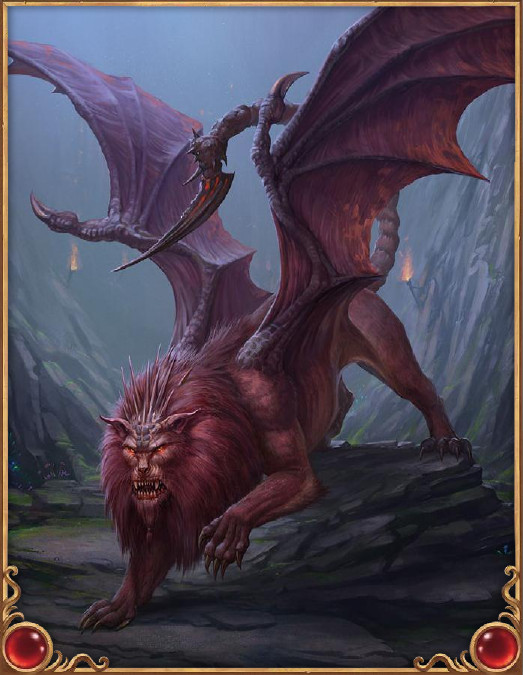
\includegraphics[scale=1]{\art/manticore.jpg}

\end{multicols*}


\addsection{Strech Goals Neutral}{\covers/stretch_goals_neutral.jpg}

\begin{multicols*}{2}

\footnotesize

\begin{itemize}[leftmargin=0pt, label={}, noitemsep, noitemsep]
  \item \textbf{\small{\underline{Miniatures}}} (47)
  \item
  \item \textbf{Neutral Unit} (15)
  \item Azure Dragons (1)
  \item Boars (1)
  \item Crystal Dragons (1)
  \item Diamond Golems (1)
  \item Enchanters (1)
  \item Faerie Dragons (1)
  \item Gold Golems (1)
  \item Halflings (1)
  \item Mummies (1)
  \item Nomads (1)
  \item Peasants (1)
  \item Rogues (1)
  \item Rust Dragons (1)
  \item Sharpshooters (1)
  \item Trolls (1)
  \item
  \item \textbf{Towns} (6)
  \item Castle (1)
  \item Dungeon (1)
  \item Fortress (1)
  \item Necropolis (1)
  \item Ramparts (1)
  \item Tower (1)
  \item
  \item \textbf{Others} (21)
  \item 5 Valuables (5)
  \item Campfire (4)
  \item Dragon Utopia (1)
  \item Grail (1)
  \item Morale (5)
  \item Round Tracker (1)
  \item Treasure Chests (4)
  \item
  \item \textbf{\small{\underline{Plastic Tokens}}} (81)
  \item
  \item 1 Valuable (10)
  \item 3 Valuables (6)
  \item 1 Building Material (9)
  \item 3 Building Material (12)
  \item 10 Building Material (5)
  \item 1 Gold (11)
  \item 3 Gold (13)
  \item 10 Gold (10)
  \item 20 Gold (5)
\end{itemize}

\columnbreak

\hspace{-2.75em}
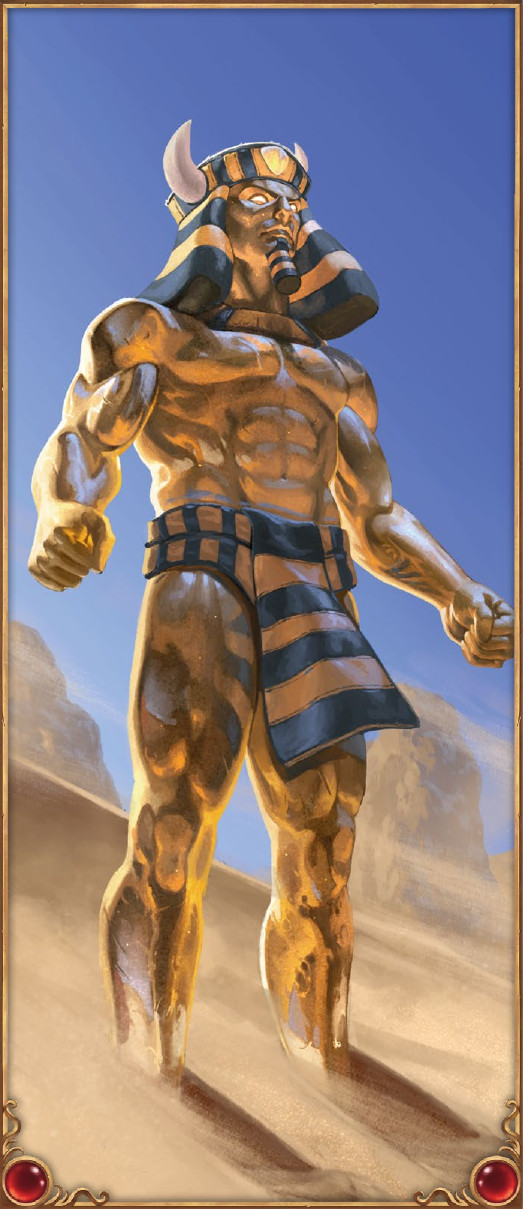
\includegraphics[scale=1]{\art/gold_golem.jpg}

\end{multicols*}


\addsection{Battlefield}{\covers/battlefield.jpg}

\begin{multicols}{3}

\footnotesize

\begin{itemize}[leftmargin=0pt, label={}, noitemsep, noitemsep]
  \item \textbf{\small{\underline{Books Leaflets}}} (3)
  \item
  \item Battlefield Rulebook (1)
  \item Player's Aid Battlefield (2)
\end{itemize}

\begin{itemize}[leftmargin=0pt, label={}, noitemsep, noitemsep]
  \item \textbf{\small{\underline{Boards}}} (1)
  \item
  \item Battlefield (1)
\end{itemize}

\begin{itemize}[leftmargin=0pt, label={}, noitemsep, noitemsep]
  \item \textbf{\small{\underline{Obstacle Tokens}}} (10)
  \item
  \item Fire (2)
  \item Lake/Lake (1)
  \item Log/Castle Wall (2)
  \item Rock/Castle Wall (1)
  \item Skeleton, Stump/Castle Gate (1)
  \item Skeleton/Skeleton (1)
  \item Skull, Rock/Skull, Rock (1)
  \item Skull/Caste Wall (1)
\end{itemize}

\textbf{\small{\underline{Initiative Tokens}}} (1)

\vspace*{\fill}
\columnbreak

\begin{itemize}[leftmargin=0pt, label={}, noitemsep, noitemsep]
  \item \textbf{\small{\underline{Cards}}} (70)
  \item
  \item \textbf{Adventure Cards} (50)
  \item Campfire (2)
  \item Corpse (2)
  \item Crypt (2)
  \item Cyclops Stockpile (2)
  \item Dragon Utopia (2)
  \item Dwarven Treasury (2)
  \item Imp Cache (2)
  \item Learning Stone (2)
  \item Magic Spring (2)
  \item Obelisk (4)
  \item Pandora's Box (2)
  \item Scholar (2)
  \item Shrine of Magic Gesture (2)
  \item Spell Scroll (2)
  \item Temple (2)
  \item Trading Post (6)
  \item Treasure Chest (2)
  \item Tree of Knowledge (2)
  \item Warrior's Tomb (2)
  \item Water Wheel (2)
  \item Windmill (2)
  \item Witch Hut (2)
\columnbreak
  \item \textbf{Negative Morale Cards} (10)
  \item Attack set one to -1 (1)
  \item Discard 1 card at random (2)
  \item Paralyse one unit (1)
  \item Reroll +1 on attack die (2)
  \item Roll one less die when doing 2 search or 2 treasure (1)
  \item Search(x) is search(1) (1)
  \item Skip unit activation on -1 attack die (1)
  \item Suffer -1 to next attack, defense or power roll (1)
  \item
  \item \textbf{Positive Morale Cards} (10)
  \item Remove paralyse one unit (1)
  \item +1 attack, +1 defense or +1 power on next combat (1)
  \item Discard an adventurer card and draw another (1)
  \item Discard any number of cards and draw as many (1)
  \item Do another search(x) (1)
  \item Draw a card on combat start (2)
  \item Next attack set a die to +1 (1)
  \item Reroll a die (2)
  \item
  \item \textbf{Other} (1)
  \item Battlefield Deck Cards (1)
\end{itemize}

\end{multicols}

\vfill
\begin{center}
  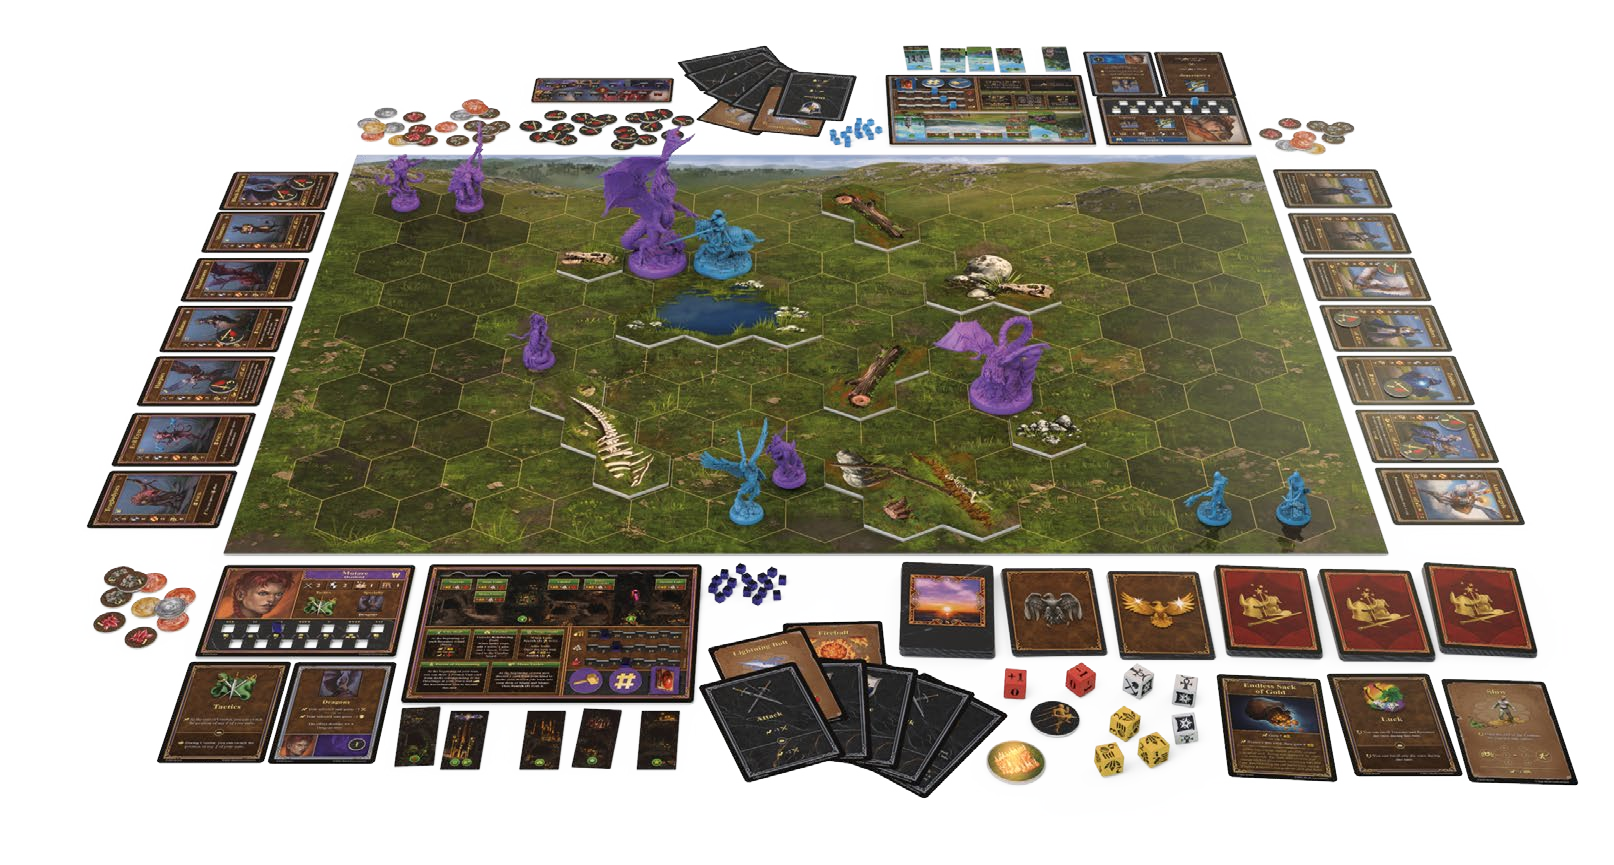
\includegraphics[width=0.9\linewidth]{\images/battlefield.png}
\end{center}


\end{document}
